\documentclass{standalone}
\usepackage{tikz}
\usetikzlibrary{patterns, positioning}


\begin{document}
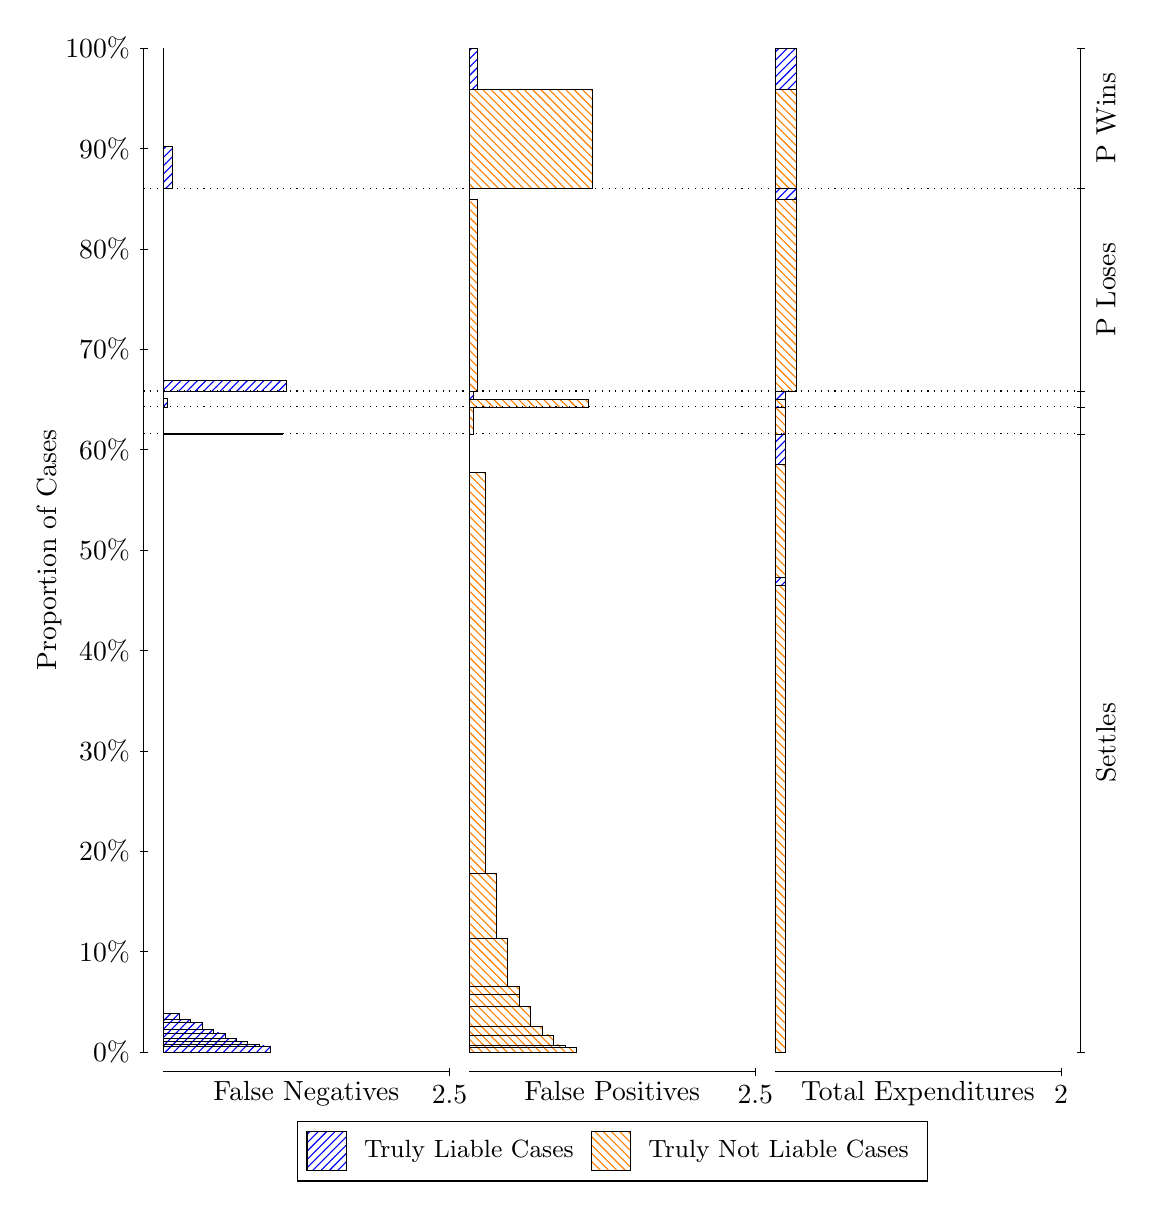
\begin{tikzpicture}
\draw[black, very thin] (1.5,1.75) -- (1.5,14.5);
\node[rotate=90, text=black, anchor=center] at (0.3, 8.125) {Proportion of Cases};
\draw[black, very thin] (1.45,1.75) -- (1.55,1.75);
\node[text=black, anchor=east] at (1.45, 1.75) {0\%};
\draw[black, very thin] (1.45,3.025) -- (1.55,3.025);
\node[text=black, anchor=east] at (1.45, 3.025) {10\%};
\draw[black, very thin] (1.45,4.3) -- (1.55,4.3);
\node[text=black, anchor=east] at (1.45, 4.3) {20\%};
\draw[black, very thin] (1.45,5.575) -- (1.55,5.575);
\node[text=black, anchor=east] at (1.45, 5.575) {30\%};
\draw[black, very thin] (1.45,6.85) -- (1.55,6.85);
\node[text=black, anchor=east] at (1.45, 6.85) {40\%};
\draw[black, very thin] (1.45,8.125) -- (1.55,8.125);
\node[text=black, anchor=east] at (1.45, 8.125) {50\%};
\draw[black, very thin] (1.45,9.4) -- (1.55,9.4);
\node[text=black, anchor=east] at (1.45, 9.4) {60\%};
\draw[black, very thin] (1.45,10.675) -- (1.55,10.675);
\node[text=black, anchor=east] at (1.45, 10.675) {70\%};
\draw[black, very thin] (1.45,11.95) -- (1.55,11.95);
\node[text=black, anchor=east] at (1.45, 11.95) {80\%};
\draw[black, very thin] (1.45,13.225) -- (1.55,13.225);
\node[text=black, anchor=east] at (1.45, 13.225) {90\%};
\draw[black, very thin] (1.45,14.5) -- (1.55,14.5);
\node[text=black, anchor=east] at (1.45, 14.5) {100\%};

\draw[black, very thin] (13.4,1.75) -- (13.4,14.5);
\draw[black, very thin] (13.35,1.75) -- (13.45,1.75);
\node[anchor=west] at (13.35, 1.75) {};
\draw[black, very thin] (13.35,9.5996) -- (13.45,9.5996);
\node[anchor=west] at (13.35, 9.5996) {};
\draw[black, very thin] (13.35,9.9422) -- (13.45,9.9422);
\node[anchor=west] at (13.35, 9.9422) {};
\draw[black, very thin] (13.35,10.144) -- (13.45,10.144);
\node[anchor=west] at (13.35, 10.144) {};
\draw[black, very thin] (13.35,12.72) -- (13.45,12.72);
\node[anchor=west] at (13.35, 12.72) {};
\draw[black, very thin] (13.35,14.5) -- (13.45,14.5);
\node[anchor=west] at (13.35, 14.5) {};

\draw[black, very thin, pattern color=blue, pattern=north east lines] (1.75,1.75) rectangle (3.1125,1.8284);
\draw[black, very thin, pattern color=blue, pattern=north east lines] (1.75,1.8284) rectangle (2.9672,1.8511);
\draw[black, very thin, pattern color=blue, pattern=north east lines] (1.75,1.8511) rectangle (2.8218,1.889);
\draw[black, very thin, pattern color=blue, pattern=north east lines] (1.75,1.889) rectangle (2.6765,1.9222);
\draw[black, very thin, pattern color=blue, pattern=north east lines] (1.75,1.9222) rectangle (2.5312,1.992);
\draw[black, very thin, pattern color=blue, pattern=north east lines] (1.75,1.992) rectangle (2.3858,2.0385);
\draw[black, very thin, pattern color=blue, pattern=north east lines] (1.75,2.0385) rectangle (2.2405,2.1277);
\draw[black, very thin, pattern color=blue, pattern=north east lines] (1.75,2.1277) rectangle (2.0952,2.1676);
\draw[black, very thin, pattern color=blue, pattern=north east lines] (1.75,2.1676) rectangle (1.9498,2.2396);
\draw[black, very thin, pattern color=orange, pattern=north west lines] (1.75,2.2396) rectangle (1.75,9.5996);
\draw[black, very thin, pattern color=blue, pattern=north east lines] (1.75,9.5996) rectangle (3.2578,9.6084);
\draw[black, very thin, pattern color=orange, pattern=north west lines] (1.75,9.6084) rectangle (1.75,9.9422);
\draw[black, very thin, pattern color=blue, pattern=north east lines] (1.75,9.9422) rectangle (1.8045,10.051);
\draw[black, very thin, pattern color=orange, pattern=north west lines] (1.75,10.051) rectangle (1.75,10.144);
\draw[black, very thin, pattern color=blue, pattern=north east lines] (1.75,10.144) rectangle (3.3123,10.281);
\draw[black, very thin, pattern color=orange, pattern=north west lines] (1.75,10.281) rectangle (1.75,12.72);
\draw[black, very thin, pattern color=blue, pattern=north east lines] (1.75,12.72) rectangle (1.859,13.25);
\draw[black, very thin, pattern color=orange, pattern=north west lines] (1.75,13.25) rectangle (1.75,14.5);
\draw[black, very thin, pattern color=orange, pattern=north west lines] (5.6333,1.75) rectangle (6.9958,1.8049);
\draw[black, very thin, pattern color=orange, pattern=north west lines] (5.6333,1.8049) rectangle (6.8505,1.8412);
\draw[black, very thin, pattern color=orange, pattern=north west lines] (5.6333,1.8412) rectangle (6.7052,1.9663);
\draw[black, very thin, pattern color=orange, pattern=north west lines] (5.6333,1.9663) rectangle (6.5598,2.0705);
\draw[black, very thin, pattern color=orange, pattern=north west lines] (5.6333,2.0705) rectangle (6.4145,2.3264);
\draw[black, very thin, pattern color=orange, pattern=north west lines] (5.6333,2.3264) rectangle (6.2692,2.4797);
\draw[black, very thin, pattern color=orange, pattern=north west lines] (5.6333,2.4797) rectangle (6.2692,2.5859);
\draw[black, very thin, pattern color=orange, pattern=north west lines] (5.6333,2.5859) rectangle (6.1238,3.1878);
\draw[black, very thin, pattern color=orange, pattern=north west lines] (5.6333,3.1878) rectangle (5.9785,4.0218);
\draw[black, very thin, pattern color=orange, pattern=north west lines] (5.6333,4.0218) rectangle (5.8332,9.11);
\draw[black, very thin, pattern color=blue, pattern=north east lines] (5.6333,9.11) rectangle (5.6333,9.5996);
\draw[black, very thin, pattern color=orange, pattern=north west lines] (5.6333,9.5996) rectangle (5.6878,9.9333);
\draw[black, very thin, pattern color=blue, pattern=north east lines] (5.6333,9.9333) rectangle (5.6333,9.9422);
\draw[black, very thin, pattern color=orange, pattern=north west lines] (5.6333,9.9422) rectangle (7.1412,10.034);
\draw[black, very thin, pattern color=blue, pattern=north east lines] (5.6333,10.034) rectangle (5.6878,10.144);
\draw[black, very thin, pattern color=orange, pattern=north west lines] (5.6333,10.144) rectangle (5.7423,12.582);
\draw[black, very thin, pattern color=blue, pattern=north east lines] (5.6333,12.582) rectangle (5.6333,12.72);
\draw[black, very thin, pattern color=orange, pattern=north west lines] (5.6333,12.72) rectangle (7.1957,13.97);
\draw[black, very thin, pattern color=blue, pattern=north east lines] (5.6333,13.97) rectangle (5.7423,14.5);
\draw[black, very thin, pattern color=orange, pattern=north west lines] (9.5167,1.75) rectangle (9.6529,7.6723);
\draw[black, very thin, pattern color=blue, pattern=north east lines] (9.5167,7.6723) rectangle (9.6529,7.7733);
\draw[black, very thin, pattern color=orange, pattern=north west lines] (9.5167,7.7733) rectangle (9.6529,9.2111);
\draw[black, very thin, pattern color=blue, pattern=north east lines] (9.5167,9.2111) rectangle (9.6529,9.5996);
\draw[black, very thin, pattern color=orange, pattern=north west lines] (9.5167,9.5996) rectangle (9.6529,9.9333);
\draw[black, very thin, pattern color=blue, pattern=north east lines] (9.5167,9.9333) rectangle (9.6529,9.9422);
\draw[black, very thin, pattern color=orange, pattern=north west lines] (9.5167,9.9422) rectangle (9.6529,10.034);
\draw[black, very thin, pattern color=blue, pattern=north east lines] (9.5167,10.034) rectangle (9.6529,10.144);
\draw[black, very thin, pattern color=orange, pattern=north west lines] (9.5167,10.144) rectangle (9.7892,12.582);
\draw[black, very thin, pattern color=blue, pattern=north east lines] (9.5167,12.582) rectangle (9.7892,12.72);
\draw[black, very thin, pattern color=orange, pattern=north west lines] (9.5167,12.72) rectangle (9.7892,13.97);
\draw[black, very thin, pattern color=blue, pattern=north east lines] (9.5167,13.97) rectangle (9.7892,14.5);
\draw[black, dotted] (1.5,9.5996) -- (13.4,9.5996);
\draw[black, dotted] (1.5,9.9422) -- (13.4,9.9422);
\draw[black, dotted] (1.5,10.144) -- (13.4,10.144);
\draw[black, dotted] (1.5,12.72) -- (13.4,12.72);
\draw[black, very thin] (1.75,1.5) -- (5.3833,1.5);
\node[text=black, anchor=north] at (3.5667, 1.5) {False Negatives};
\draw[black, very thin] (5.3833,1.45) -- (5.3833,1.55);
\node[text=black, anchor=north] at (5.3833, 1.45) {2.5};

\draw[black, very thin] (5.6333,1.5) -- (9.2667,1.5);
\node[text=black, anchor=north] at (7.45, 1.5) {False Positives};
\draw[black, very thin] (9.2667,1.45) -- (9.2667,1.55);
\node[text=black, anchor=north] at (9.2667, 1.45) {2.5};

\draw[black, very thin] (9.5167,1.5) -- (13.15,1.5);
\node[text=black, anchor=north] at (11.333, 1.5) {Total Expenditures};
\draw[black, very thin] (13.15,1.45) -- (13.15,1.55);
\node[text=black, anchor=north] at (13.15, 1.45) {2};

\node[text=black, centered, rotate=90] at (13.72, 5.6748) {Settles};


\node[text=black, centered, rotate=90] at (13.72, 11.432) {P Loses};
\node[text=black, centered, rotate=90] at (13.72, 13.61) {P Wins};

\draw (7.449999999999999,1.5) node[draw=none] (baseCoordinate) {};
\begin{scope}[align=center]
        \matrix[scale=0.5, draw=black, below=0.5cm of baseCoordinate, nodes={draw}, column sep=0.1cm]{
            \node[rectangle, draw, minimum width=0.5cm, minimum height=0.5cm, pattern color=blue, pattern=north east lines] {}; &
            \node[draw=none, font=\small, text=black] (B) {Truly Liable Cases}; &
            \node[rectangle, draw, minimum width=0.5cm, minimum height=0.5cm, pattern color=orange, pattern=north west lines] {}; &
            \node[draw=none, font=\small, text=black] (B) {Truly Not Liable Cases}; \\
            };
\end{scope}

\end{tikzpicture}
\end{document}